\documentclass[letterpaper]{tufte-book}
\usepackage[utf8]{inputenc}
\usepackage{amsmath}  % extended mathematics
\usepackage{booktabs} % book-quality tables
\usepackage{units}    % non-stacked fractions and better unit spacing
\usepackage{multicol} % multiple column layout facilities
\usepackage{lipsum}   % filler text
\usepackage{fancyvrb} % extended verbatim environments
  \fvset{fontsize=\normalsize}% default font size for fancy-verbatim environments
\usepackage{xspace}
\usepackage{graphicx}
\usepackage{hyperref}

\setkeys{Gin}{width=\linewidth,totalheight=\textheight,keepaspectratio}

\title{Homework 03 Questions. PLS206 Fall 2013}
\author{Emilio A. Laca}

\usepackage{Sweave}
\begin{document}

\setkeys{Gin}{width=1.1\marginparwidth} %% Sweave

\maketitle


\begin{Schunk}
\begin{Sinput}
> t <- rnorm(100)
\end{Sinput}
\end{Schunk}
%% a margin figure

\begin{marginfigure}
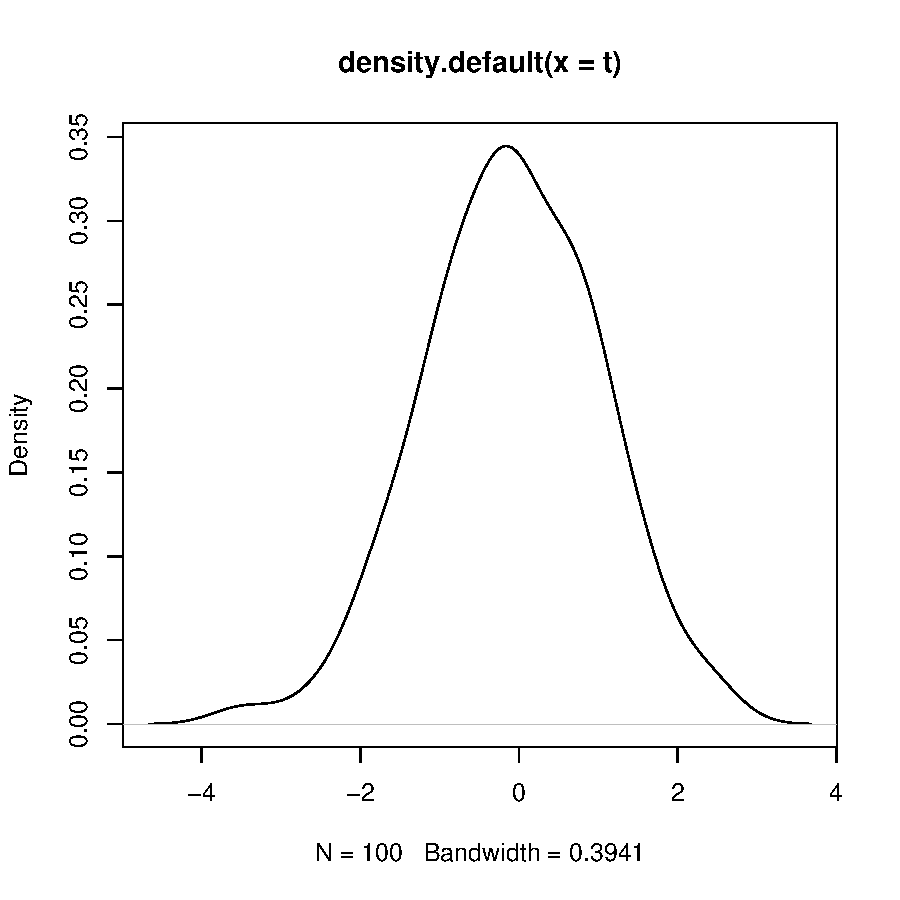
\includegraphics{QuestionsHW03-003}
\end{marginfigure}



\end{document}
